% !TEX program = lualatex
% Generated by new_lecture_note.sh
\documentclass[11pt]{article}

\usepackage{fontspec}
\usepackage{microtype}
\usepackage{mathtools,amssymb,amsfonts,amsthm,bm}
\usepackage{tikz}
\usepackage{enumitem}
\usepackage{xcolor}
\usepackage{booktabs,array,xcolor}
\usepackage{geometry,fancyhdr,setspace}
\usepackage[hidelinks]{hyperref}
\usepackage[nameinlink,noabbrev]{cleveref}

\geometry{margin=1in,headheight=15pt}
\setstretch{1.12}
\setlength{\parindent}{0pt}
\setlength{\parskip}{0.55em plus 0.12em minus 0.08em}
\setlength{\abovedisplayskip}{0.8em plus 0.2em minus 0.1em}
\setlength{\belowdisplayskip}{0.8em plus 0.2em minus 0.1em}
\allowdisplaybreaks[3]
\setlist{leftmargin=*,topsep=0.35em,itemsep=0.15em,parsep=0pt}

% ---------- Metadata ----------
\newcommand{\studentname}{Keshav Ramamurthy}
\newcommand{\coursename}{Math 118}
\newcommand{\lecturenumber}{02}
\newcommand{\lecturetitle}{Lecture 02}
\newcommand{\lecturedate}{\today}

% ---------- Reusable notation ----------
\newcommand{\N}{\mathbb{N}}
\newcommand{\Z}{\mathbb{Z}}
\newcommand{\Q}{\mathbb{Q}}
\newcommand{\R}{\mathbb{R}}
\newcommand{\C}{\mathbb{C}}
\newcommand{\F}{\mathbb{F}}
\newcommand{\K}{\mathbb{K}}
\newcommand{\E}{\mathbb{E}}
\newcommand{\Prob}{\mathbb{P}}
\newcommand{\1}{\mathbf{1}}
\newcommand{\eps}{\varepsilon}
\newcommand{\dd}{\,\mathrm{d}}
\newcommand{\abs}[1]{\left\lvert#1\right\rvert}
\newcommand{\norm}[1]{\left\lVert#1\right\rVert}
\newcommand{\ip}[2]{\left\langle#1,#2\right\rangle}
\newcommand{\set}[1]{\left\{#1\right\}}
\newcommand{\given}{\,\middle\vert\,}
\newcommand{\indep}{\perp\!\!\!\perp}
\newcommand{\lto}{\longrightarrow}
\newcommand{\deriv}[2]{\frac{\mathrm{d}#1}{\mathrm{d}#2}}
\newcommand{\pderiv}[2]{\frac{\partial#1}{\partial#2}}
\DeclareMathOperator{\Aut}{Aut}
\DeclareMathOperator{\Hom}{Hom}
\DeclareMathOperator{\Ker}{ker}
\DeclareMathOperator{\im}{im}
\DeclareMathOperator{\rank}{rank}
\DeclareMathOperator{\nullity}{nullity}
\DeclareMathOperator{\Span}{span}
\DeclareMathOperator{\Var}{Var}
\DeclareMathOperator{\Cov}{Cov}

% ---------- Note environments ----------
\newtheoremstyle{notestyle}{0.7em}{0.7em}{\itshape}{}{}{\bfseries}{.5em}{}
\theoremstyle{notestyle}
\newtheorem{theorem}{Theorem}[section]
\newtheorem{lemma}[theorem]{Lemma}
\newtheorem{proposition}[theorem]{Proposition}
\newtheorem{corollary}[theorem]{Corollary}
\theoremstyle{definition}
\newtheorem{definition}[theorem]{Definition}
\newtheorem{example}[theorem]{Example}
\newtheorem{remark}[theorem]{Remark}
\newenvironment{claim}{\par\noindent\textbf{Claim.}\ }{\par}
\newenvironment{idea}{\par\noindent\textit{Idea.}\ }{\par}
\newenvironment{proofsketch}{\par\noindent\textbf{Proof sketch.}\ }{\par}

% ---------- Header ----------
\pagestyle{fancy}
\fancyhf{}
\fancyhead[L]{\coursename}
\fancyhead[C]{\lecturetitle}
\fancyhead[R]{\studentname}
\fancyfoot[C]{\thepage}

\title{\vspace{-1.5em}\textbf{\coursename -- \lecturetitle}}
\author{\studentname}
\date{\lecturedate}

\begin{document}
\maketitle

\section{Norms, Inner Products, Cauchy, etc}
\begin{definition}[norm]
\label{def:label}
A norm on a vector space V is a mapping $||. || : V \rightarrow [0, \infty).$
with properties 
\begin{itemize}
    \item Triangle Inequality: $||u + v|| \le ||u|| + ||v||.$
    \item Homogeneity $||\alpha u|| = |\alpha| ||u||$
    \item Positive Definiteness. $||u|| = 0 \iff u = 0$
    \item Distance from u and v is $||u-v||$
\end{itemize}
\end{definition}
\subsection{Norms on $R^n$ or $C^n$}
\begin{itemize}
    \item One-norm: $||x||_{1} = \sum_{k=1}^{n} |x_k|$
    \item  Two-norm: $||x||_{2} = \sqrt{\sum_{k=1}^{n}(x_k)^2}$
    \item Max-norm: $||x||_{\infty} = \max_{k \le n} |x_k|$
\end{itemize}
\begin{definition}[Unit Ball]
\label{def:label}
$B = \{x \in V : ||x|| \le 1\}$
\end{definition}
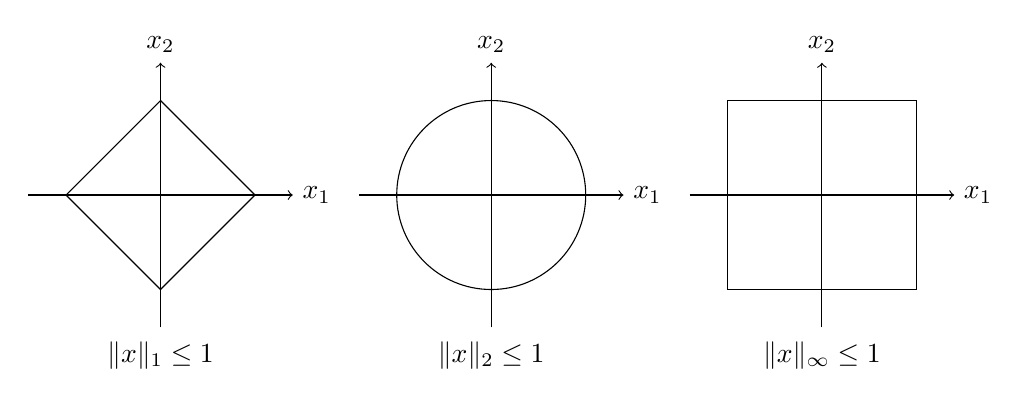
\begin{tikzpicture}[scale=1.2]
    % 1-norm
    \draw[->] (-1.4,0) -- (1.4,0) node[right] {$x_1$};
    \draw[->] (0,-1.4) -- (0,1.4) node[above] {$x_2$};
    \draw (1,0) -- (0,1) -- (-1,0) -- (0,-1) -- cycle;
    \node at (0,-1.7) {$\|x\|_1 \leq 1$};

    % 2-norm
    \begin{scope}[xshift=3.5cm]
        \draw[->] (-1.4,0) -- (1.4,0) node[right] {$x_1$};
        \draw[->] (0,-1.4) -- (0,1.4) node[above] {$x_2$};
        \draw (0,0) circle (1);
        \node at (0,-1.7) {$\|x\|_2 \leq 1$};
    \end{scope}

    % infinity-norm
    \begin{scope}[xshift=7cm]
        \draw[->] (-1.4,0) -- (1.4,0) node[right] {$x_1$};
        \draw[->] (0,-1.4) -- (0,1.4) node[above] {$x_2$};
        \draw (-1,-1) rectangle (1,1);
        \node at (0,-1.7) {$\|x\|_\infty \leq 1$};
    \end{scope}
\end{tikzpicture}
\par For any $ x\in \mathbb{C}^{n}$, we have $$||x||_{\infty} \le ||x||_2 \le ||x||_1$$
because $$|x||_{\infty} = \sqrt{\max_{k} |x_k|^2} \le \sqrt{\sum_{k} |x_k|^2}$$
% \textit{Write the one-sentence point of today's lecture here.}
\[
x =
\begin{pmatrix}
x_1\\
x_2\\
\vdots\\
x_n
\end{pmatrix},
\qquad
e_j =
\begin{pmatrix}
0\\
\vdots\\
0\\
1\\
0\\
\vdots\\
0
\end{pmatrix}
\quad
\text{($1$ in the $j$th slot)}
\]
where $(e_j)_i = S_{ij} =
\begin{cases}
1, & i=j,\\
0, & i\ne j.
\end{cases}$
\par So we can rewrite $$||x||_2 = ||x_1e_1 + x_2 e_2 + \cdots + x_n e_n||_2$$
By the triangle inequality we have 
$$ ||x_1e_1 + x_2 e_2 + \cdots + x_n e_n||_2 \le ||x_1e_1||_2 + ||x_2e_2||_2 + \cdots +
||x_ne_n||_2$$
$$||x_1e_1||_2
+  \cdots + ||x_ne_n||_2 = |x_1|||e_1||_2 + |x_2|||e_2||_2 + \cdots + |x_n| ||e_n||_2$$
Notice by definition of $e_i$ its two norm would be 1, so this is just $\sum_{i} |x_k| =
||x||_1$
\begin{remark}[Unit Balls Nested in the opposite direction]
\label{rem:label}
We have $$B_1 \subseteq B_2 \subseteq B_{\infty}$$

\[
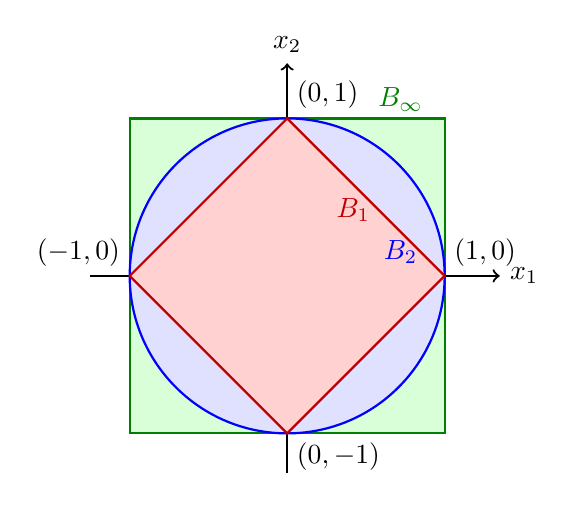
\begin{tikzpicture}[scale=2]

    % Axes
    \draw[->, thick] (-1.25,0) -- (1.35,0) node[right] {$x_1$};
    \draw[->, thick] (0,-1.25) -- (0,1.35) node[above] {$x_2$};

    % B_infinity
    \fill[green!15] (-1,-1) rectangle (1,1);
    \draw[thick, green!50!black] (-1,-1) rectangle (1,1);

    % B_2
    \fill[blue!12] (0,0) circle (1);
    \draw[thick, blue] (0,0) circle (1);

    % B_1
    \fill[red!18] 
        (1,0) -- (0,1) -- (-1,0) -- (0,-1) -- cycle;
    \draw[thick, red!75!black]
        (1,0) -- (0,1) -- (-1,0) -- (0,-1) -- cycle;

    % Coordinate labels
    \node[above right] at (1,0) {$(1,0)$};
    \node[above left] at (-1,0) {$(-1,0)$};
    \node[above right] at (0,1) {$(0,1)$};
    \node[below right] at (0,-1) {$(0,-1)$};

    % Ball labels
    \node[red!75!black] at (0.42,0.42) {$B_1$};
    \node[blue] at (0.72,0.15) {$B_2$};
    \node[green!50!black] at (0.72,1.12) {$B_\infty$};

\end{tikzpicture}
\]
\par if $x \in B$, then $||x||_1 \le 1$ so $$||x||_2 \le ||x||_1 \le 1$$
\end{remark}
\section{Inner Products}
An inner product is a mapping $\langle ., . \rangle : V x V \rightarrow \mathbb{C}$ such
that 
\begin{enumerate}
    \item $\langle u, u\rangle > u \text{ if } x \ne 0$
    \item $\langle v, u\rangle = \overline{\langle u, v \rangle}$
    \item $\langle \alpha u, v\rangle = \alpha \langle u, v \rangle.$
    \item $\langle u + v, w\rangle = \langle u, w\rangle + \langle v, w\rangle$
    \item 3 implies that $\langle 0, v\rangle = 0$
    \item 2 and 3 imply that $\langle u, \alpha v\rangle = \overline{\alpha}\langle u,
        v\rangle$ 
    % \item $(\langle, .)$ is a sesquilinear form) $$\overline{\alphakj
    \item 2 and 4 imply that $\langle w, u + v \rangle = \langle w, u \rangle + \langle
        w, v\rangle$
\end{enumerate}
Geometrically: $$\langle u, v \rangle = ||u|| \cdot ||v|| \cdot \cos \theta$$
\section{Definitions and notation}
\begin{definition}[First definition]
Write the definition and one sentence explaining why it matters.
\end{definition}

\section{Claims, theorems, and proof sketches}
\begin{claim}
State the claim in one precise sentence.
\end{claim}

\begin{proofsketch}
Record the key idea, the first useful equation, and the step that still needs checking.
\end{proofsketch}

\section{Examples and calculations}
\begin{example}[Lecture example]
Write the setup, the calculation, and the conclusion.
\end{example}

\section{Questions and follow-up}
\begin{itemize}
  \item What is still unclear?
  \item Which exercise or reading should I revisit?
  \item TODO: 
\end{itemize}

\end{document}
